\section{Theorie}
\label{sec:Theorie}
Um Röntgenstrahlung zu erzeugen wird mithilfe einer Glühkathode Elektronen emittiert und auf eine Anode hin beschleunigt.
Treffen die Elektronen auf die Anode entsteht Röntgenstrahlung.
\\
Das Elektron wird im Coulombfeld des Atoms gebremst (kontinuierliches Bremsspektrum).
Dabei wird ein Photon abgegeben, dessen Energie der des Elektrons abgegebenen Energie entspricht.
\\
Das charakteristische Spektrum beschreibt wie ein Elektron aus der äußeren $m$-ten Schale durch die Ionisierung des Anodenmaterials in die innere $n$-te Schale springt.
Bei diesem Prozess wird ein Photon abgegeben, dessen Energie die Energiedifferenz
\begin{equation}
    h \cdot \nu = E_m - E_n
    \label{eqn:bindungsenergie}
\end{equation}
der beiden Atomschalen entspricht.
Das charakteristische Spektrum besteht daher aus scharfen Linien, dessen Energie abhängig von dem Anodenmaterial ist.
Die Linien werden als $K_\alpha$, $K_\beta$, $L_\alpha$, $...$ bezeichnet, wobei $k, L, M$ die Schale auf die das Elektron wechselt bezeichnet.
Die Schale aus der das Elektron stammt wird mit $\alpha$, $\beta$, $...$ gekennzeichnet.
\\
Atome mit mehreren Elektronen haben nach außen hin eine geringere positive Ladung, da die Hüllenelektronen die Kernladung abschirmen.
Dadurch wirkt auf das äußere Elektron eine geringere Coulomb-Kraft.
Die Bindungsenergie $E_n$ eines Elektron auf der $n$-ten Schale berechnet sich nach
\begin{equation*}
    E_n = - R_\infty \cdot z_\text{eff}^2 \cdot \frac{1}{n^2}
\end{equation*}
mit der effektiven Kernladung $z_\text{eff} = z - \sigma$, der Rydbergenergie $R_\infty = \SI{13.6}{\electronvolt}$ und der Abschirmkonstante $\sigma$.
Die Elektronen besitzen nicht die selbe Bindungsenergien, da sie nicht den gleichen Bahndrehimpuls und Elektronenspin aufweisen.
Daher ist jede charakteristische Linie in nebeneinander liegenden Linien aufgelöst, die in diesem Versuch nicht aufgespalten werden können.
Dies wird auch als Feinstruktur bezeichnet.
Die K-Linien werden von der Bremsstrahlung überlagert.
\\
Bei niedrigen Energien ($E < \SI{1}{\mega\electronvolt}$) dominiert der Compton- und Photoeffekt.
Steigt die Energie so nimmt der Absorptionskoeffizient ab, bis die Photoenergie gerade größer als die Bindungsenergie ist \eqref{eqn:bindungsenergie}.
Dann steigt der Absorptionskoeffizient sprunghaft an (Absorptionskante).
Mithilfe der Sommerfeldschen Feinstrukturformel kann die Bindungsenergie unter Brücksichtung der Feinstruktur berechnet werden.
Aus der Formel folgt für Elektronen aus der K-Schale (n=1) die Abschirmkonstante
\begin{equation}
    \sigma_K = Z - \sqrt{\frac{E_K}{R_\infty} - \frac{\alpha^2 Z^4}{4}} .
    \label{eqn:abschirm_k}
\end{equation}
Für die Elektronen aus der L-Kante kann nach
\begin{equation}
    \sigma_L = Z - \left( \frac{4}{\alpha}\sqrt{\frac{\Delta E_L}{R_\infty} - \frac{5 \Delta E_L}{R_\infty}} \right) \cdot \left (1 + \frac{19}{32}\alpha^2 \frac{\Delta E_L}{R_\infty}  \right)
    \label{eqn:abschirm_l}
\end{equation}
die Abschirmkonstante bestimmt werden.
Zur Berechnung wird die Energiedifferenz $\Delta E_\text{L} = E_\text{L,II} - E_\text{L,III}$, die Ordnungszahl Z, die konstante Rydbergenergie $R_\infty$ und die Feinstrukturkonstante $\alpha$ benötigt.
Mithilfe der Bragg'schen Reflexion 
\begin{equation}
    2 d \sin \alpha = n \lambda
    \label{eqn:lambdaalpha}
\end{equation}
kann die Wellenlänge $\lambda$ bei bestimmter Beugungsordnung $n$ bestimmt werden.
\begin{figure}
    \centering
    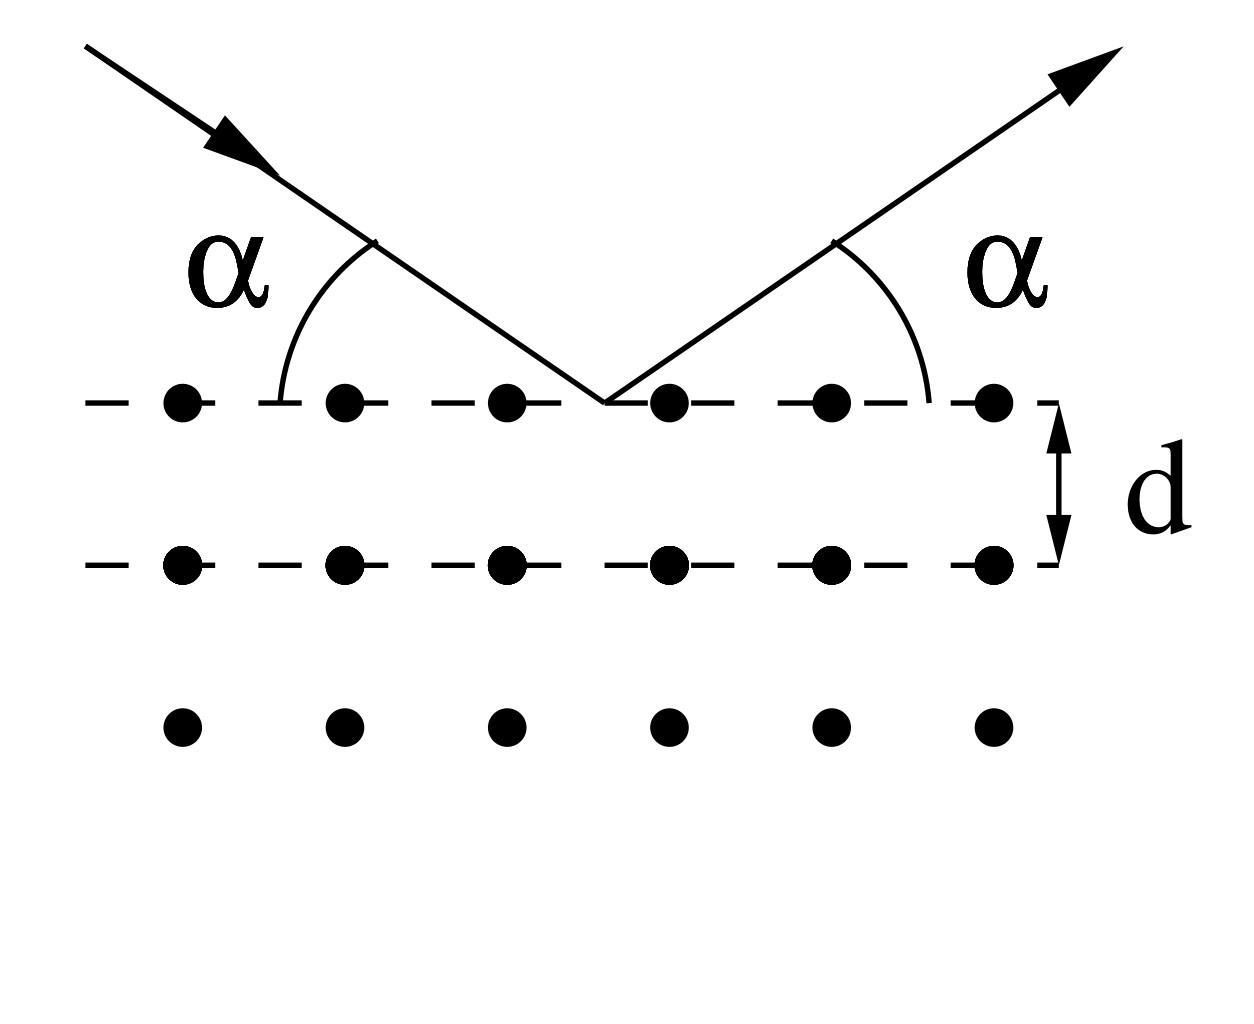
\includegraphics[width=0.3\textwidth]{content/data/kristall.jpg}
    \caption{Bragg'sche Reflexion graphisch dargestellt. \cite[3]{anleitung}}
    \label{fig:bragg}
\end{figure}
Fällt Röntgenlicht auf ein 3D-Gitter, so werden die Photonen an jedem Atom des Gitters gebeugt (siehe Abb. \ref{fig:bragg}).
Bei einem bestimmten Winkel $\alpha$, werden die Wellen perfekt überlagert (konstruktive Interferenz).
Die Gitterkonstante kann hier als $d_\text{LiF}=\SI{201.4}{\pico\metre}$ angenommen werden.
\\
Die Abschirmkonstanten können aus den Emissionsenergien der $K_\alpha$ und $K_\beta$-Linie abgeschätzt werden:
\begin{equation}
    \sigma_1 = z - \sqrt{\frac{E_\text{abs}}{R_\infty}}
    \label{eqn:sigma1}
\end{equation}
\begin{equation}
    \sigma_2 = z - \sqrt{\frac{m^2}{n^2} \left( z - \sigma_1 \right)^2 - \frac{E_{k,\alpha}}{R_\infty}m^2}
    \label{eqn:sigma2}
\end{equation}
\begin{equation}
    \sigma_3 = z - \sqrt{\frac{l^2}{n^2} \left( z - \sigma_1 \right)^2 - \frac{E_{k,\beta}}{R_\infty}l^2}
    \label{eqn:sigma3}
\end{equation}
Es gilt $n=1$, $m=2$ und $l=3$.
\\
Die Halbwertsbreite (FWHM) bezeichnet die Breite einer Kurve bei ihrem halben Maximum.
Sie wird im folgenden als $\Delta E_\text{FWHM}$ bezeichnet und zur Berechnung des Auflösungsvermögen
\begin{equation}
    A = \frac{E_\text{K}}{\Delta E_\text{FWHM}}
    \label{eqn:aufloesung}
\end{equation}
verwendet.
\\
Das Moseley'sche Gesetz
\begin{equation}
    E_\text{K} = R h (z - \sigma )^2
    \label{eqn:moseley}
\end{equation}
wird zur Berechnung der Rydbergfrequenz $R$ benötigt.
Aus der Rydbergfrequenz kann dann die Konstante $R_\infty = h \cdot R$ (Rydbergenergie) bestimmt werden.